\documentclass{exam}
\setlength{\parskip}{0pt}
\setlength{\parindent}{0pt}
\setlength{\voffset}{-15pt}
\usepackage[onehalfspacing]{setspace} % Sets Spacing to 1.5
\usepackage[utf8]{inputenc} % Use UTF-8 encoding
\usepackage{float} % Improved interface for floating objects
\usepackage[colorlinks = true,
            linkcolor = blue,
            urlcolor  = blue,
            citecolor = blue,
            anchorcolor = blue]{hyperref} % For hyperlinks in the PDF
\usepackage{graphicx, multicol} % Enhanced support for graphics
\usepackage{amsmath}
\usepackage{framed, caption}
\usepackage{array}
\usepackage{float}
\usepackage{amsmath}
\usepackage{bbm}
\newcommand\tab[1][0.2cm]{\hspace*{#1}}
\usepackage{multicol}
%----------------------------------------------------------------------------------------
\begin{document}

\begin{minipage}{0.295\textwidth} % Left side of title section
\raggedright
SIL765 - Net. \& Sys. Security\\ % Your lecture or course
\footnotesize % Authors text size
CSE, IIT Delhi (SEM2, 2020-21) % Department
\medskip\hrule
\end{minipage}
\begin{minipage}{0.4\textwidth} % Center of title section
\centering 
\large % Title text size
\textbf{Assignment 1}\\ % Assignment number
\normalsize % Subtitle text size
 % Assignment subtitle
\end{minipage}
\begin{minipage}{0.295\textwidth} % Right side of title section
\raggedleft
2018CS10388\\ % Entry Number
\footnotesize
Sharique Shamim % Name
\medskip\hrule
\end{minipage}
\vspace{0.1in}
\section{Cracking RSA}
To run the script do: (Note here python2 has been used)
\begin{center}
    \texttt{cd problem-3},
    \texttt{python2 crack.py n}
\end{center}
RSA Algorithm is an asymmetric cryptography algorithm. The algorithm makes use of Public Key and Private Key. Messages encrypted through public key can only be correctly decrypted through private key. As the name describes the public key is given to everyone and the private key is kept private. \vspace{0.05in} \\
\textbf{Idea of RSA Algorithm}: \vspace{0.05in} \\
RSA algorithm is based on the fact that it is very difficult to factorize large integers. The public key consists of two numbers where one number is multiplication of two large prime numbers. And private key is also derived from the same two prime numbers. So if somebody can factorize the large number, the private key is compromised. Therefore encryption strength totally lies on the key size and if we double or triple the key size, the strength of encryption increases exponentially. RSA keys can be typically 1024 or 2048 bits long, but experts believe that 1024 bit keys could be broken in the near future. But till now it seems to be an infeasible task. \vspace{0.05in} \\
\textbf{RSA Algorithm}:
\begin{itemize}
    \item Factorize $n$ \vspace{0.05in} \\
    \tab if $ n \le 10^{20}$ then use Pollard-Rho to factorize n otherwise use ECM to factorize n
    \item Key Setup \vspace{0.05in} \\
    \tab Obtain the prime factors $p$, $q$ such that $n = p \cdot q$ \vspace{0.05in} \\
    \tab Compute $\phi = (p - 1) \cdot (q - 1)$ \vspace{0.05in} \\
    \tab Choose an integer $e$ such that gcd($e, phi$) = $1$ \vspace{0.05in} \\
    \tab Choose an integer $d$ such that $(d \cdot e)$ mod $\phi = 1$ \vspace{0.05in} \\
    \tab Publish the public key $\{e, n\}$ \vspace{0.05in} \\
    \tab Keep the private key $\{d, n\}$
    \item Encryption \vspace{0.05in} \\
    \tab Convert the characters of the plain text to numbers. \vspace{0.05in} \\
    \tab Use the public key $K$ and compute the cipher text as $C = M^e$ mod $n$ \vspace{0.05in} \\
    \tab Convert the numbers of cipher text to characters.
    \item Decryption \vspace{0.05in} \\
    \tab Convert the characters of the cipher text to numbers. \vspace{0.05in} \\
    \tab Use the private key $K$ and compute the plain text as $M = C^d$ mod $n$ \vspace{0.05in}
\end{itemize}
\section{Time to factorize vs number of digits in n}
\begin{figure}[h]
\centering
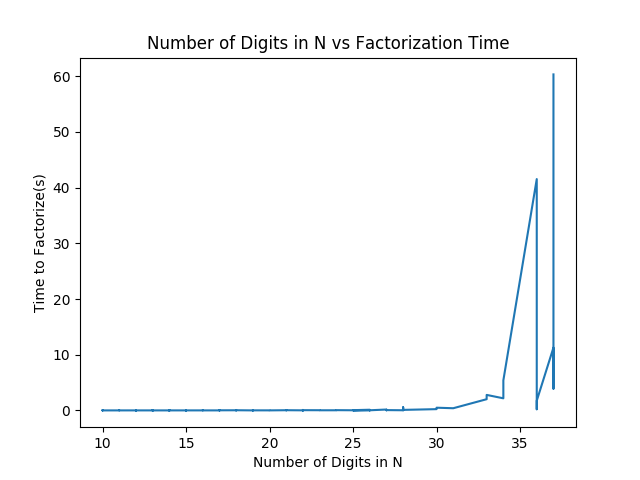
\includegraphics[scale=0.8]{rsa_plot.png}
\end{figure}
\textbf{Observations}:
In the given file 'nlist.txt' there are several numbers which are square of a prime numbers. But for RSA algorithm to decrypt the cipher text correctly both p and q should be distinct. The following are such numbers in the given file: \\
$2605796209$, $3678058609$, $3694086841$, $4303234442515849$, $961801438520428081$, $11651738070536913351684889$, $840859136266769099141989302482624329$, $1316872907073608066468826571215294289$ \vspace{0.05in} \\
\textbf{Configuration of laptop used}: Intel i5 \vspace{0.05in} \\
\textbf{Largest n cracked within 5 minutes}: All the numbers in the file are cracked within 5 minutes. Largest number of digits in the file is $37$. \vspace{0.05in} \\
\textbf{Conclusion}: The time required to factorize is very low but increases slowly when the number of digits in n increases.
\end{document}